\documentclass[12pt, a4paper]{ctexart}
\usepackage{geometry}
\geometry{left=2.5cm, right=2.5cm, top=3cm, bottom=3cm}
\usepackage{graphicx}
\usepackage{xcolor}
\usepackage{circuitikz}
\usepackage{subcaption}
\usepackage{float}
\usepackage{amsmath}
\usepackage{listings}
\usetikzlibrary{arrows, shapes.gates.logic.US, positioning}
\ctikzset{
    logic ports=ieee,
    logic ports/scale=0.8,
    multipoles/flipflop/pin spacing=0.4
}
\lstset{
    basicstyle=\ttfamily\small,
    frame=single,
    framesep=5pt,
    xleftmargin=10pt,
    xrightmargin=10pt,
    keywordstyle=\color{blue},
    commentstyle=\color{gray},
    breaklines=true
}

\begin{document}

% 封面
\begin{titlepage}
    \centering
    \vspace*{5cm}
    {\Huge\bfseries 实验报告\par}
    \vspace{2cm}
    {\Large 课程：数字逻辑与计算机组成\par}
    \vspace{1cm}
    {\Large 实验三：同步时序部件设计\par}
    \vspace{4cm}
    {\large 姓名：\underline{\makebox[4cm]{郑袭明}}\par}
    \vspace{1cm}
    {\large 学号：\underline{\makebox[4cm]{251502027}}\par}
    \vspace{1cm}
    {\large 日期：\today\par}
\end{titlepage}

\tableofcontents
\newpage

\section{实验目的}

\begin{enumerate}
    \item 掌握时序逻辑电路设计的基本方法。
    \item 掌握计数器和移位寄存器的设计方法和应用。
    \item 掌握无符号乘法器的设计方法。
    \item 掌握寄存器堆的设计方法。
    \item 掌握数字时钟的设计方法。
    \item 掌握数字系统的设计方法
\end{enumerate}

\section{实验一：4位同步计数器实验}

\subsection{整体方案设计}

本实验为单模块，逻辑如下

\begin{lstlisting}[language=Verilog, caption={4位同步计数器模块}]
module CNTR4U (
    input  wire       clk,
    input  wire       CLR,
    input  wire       LD,
    input  wire       ENP,
    input  wire       ENT,
    input  wire [3:0] D,
    output reg  [3:0] Q,
    output wire       RCO
);

  always @(posedge clk)
    if (CLR) Q <= 4'h0;
    else if (LD) Q <= D;
    else if (ENP && ENT) Q <= Q + 1'b1;
    else Q <= Q;
  assign RCO = (Q == 4'hf) && ENT;

endmodule
\end{lstlisting}

其中的分支逻辑可用逻辑门实现。

\begin{table}[H]
    \centering
    \begin{tabular}{|c|c|}
        \hline
        引脚 & 功能 \\
        \hline
        clk & 时钟信号 \\
        CLR & 同步清零 (高电平有效) \\
        LD  & 同步置数 (高电平有效) \\
        ENP & 计数使能 P \\
        ENT & 计数使能 T \\
        D   & 4位并行数据输入 \\
        Q   & 4位数据输出 \\
        RCO & 进位输出 \\
        \hline
    \end{tabular}
    \caption{4位同步计数器引脚功能表}
\end{table}

\subsection{电路设计}

\begin{figure}[H]
    \centering
    \subcaptionbox{原理图}{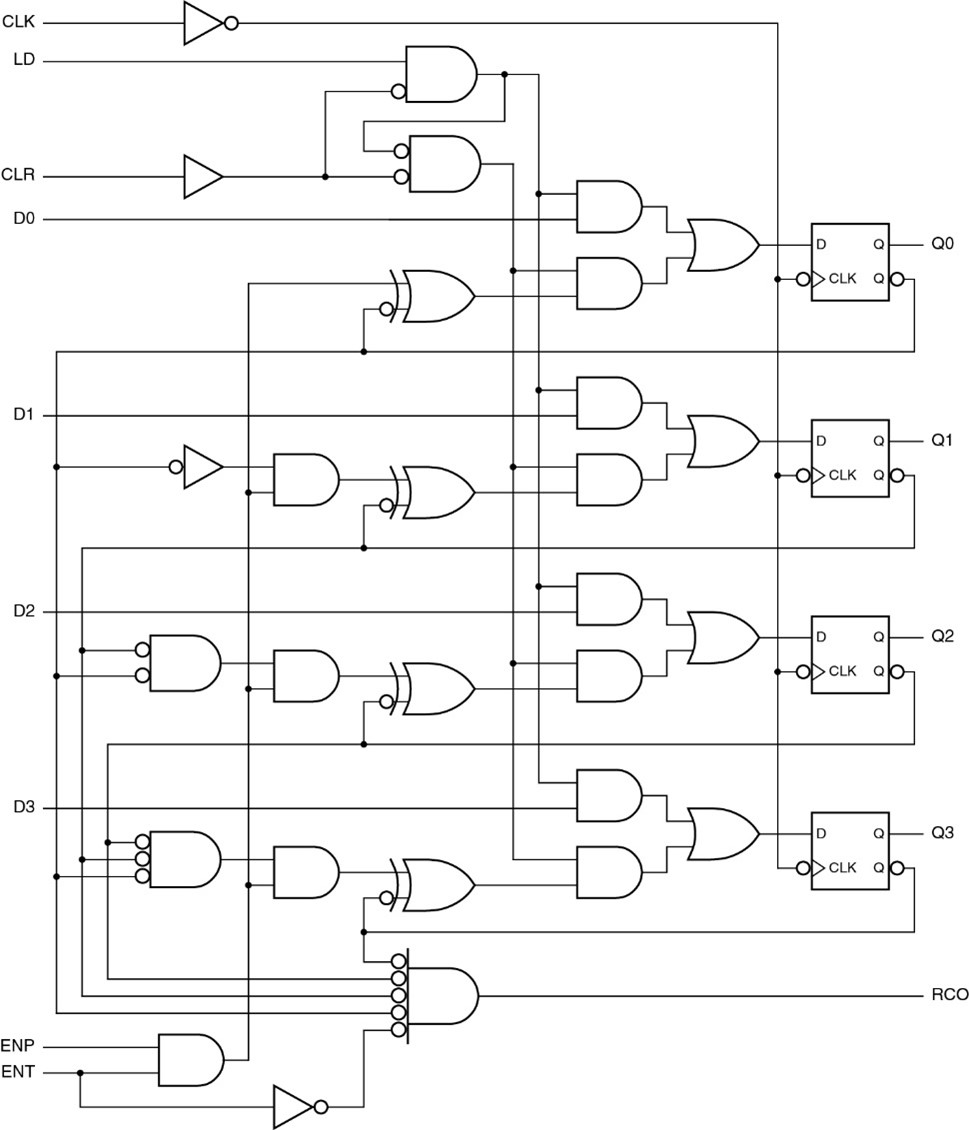
\includegraphics[width=0.5\textwidth]{assets/exp1/sch.png}}
    \subcaptionbox{电路图}{
\includegraphics[width=0.45\textwidth]{assets/exp1/circuit.png}}
    \caption{4位同步计数器电路设计}
\end{figure}

\subsection{仿真结果}

\begin{figure}[H]
    \centering
    
\includegraphics[width=\textwidth]{assets/exp1/sim1.png}
    \caption{4位同步计数器仿真结果(a)}
\end{figure}

\begin{figure}[H]
    \centering
    
\includegraphics[width=\textwidth]{assets/exp1/sim2.png}
    \caption{4位同步计数器仿真结果(b)}
\end{figure}

\begin{figure}[H]
    \centering
    
\includegraphics[width=\textwidth]{assets/exp1/sim3.png}
    \caption{4位同步计数器仿真结果(c)}
\end{figure}

由于真值表过于复杂，这里只取部分数据展示。

\begin{table}[H]
    \centering
    \begin{tabular}{|c|c|c|c|c|c|c|c|}
        \hline
        Cnt & LD & CLR & ENP & ENT & D & Q & RCO \\
        \hline
        00  & 1  & 0   & 0   & 1   & 0 & c & 0 \\
        02  & 0  & 0   & 1   & 1   & 0 & d & 0 \\
        03  & 0  & 0   & 1   & 1   & 0 & e & 0 \\
        04  & 0  & 0   & 1   & 1   & 0 & f & 1 \\
        05  & 0  & 0   & 1   & 1   & 0 & 0 & 0 \\
        06  & 0  & 0   & 1   & 1   & 0 & 1 & 0 \\
        07  & 0  & 1   & 0   & 0   & 0 & 2 & 0 \\
        08  & 0  & 0   & 1   & 1   & 0 & 0 & 0 \\
        \hline
    \end{tabular}
    \caption{4位同步计数器真值表}
\end{table}

\subsection{错误现象及分析}

在完成实验的过程中，没有遇到任何错误。

\section{实验二：4位移位寄存器实验}

\subsection{整体方案设计}

本实验为单模块，逻辑如下

\begin{lstlisting}[language=Verilog, caption={4位移位寄存器模块}]
module shift_register (
    input  wire       CLK,
    input  wire       CLR_L,
    input  wire [1:0] S,
    input  wire       RIN,
    input  wire       LIN,
    input  wire [3:0] D,
    output reg  [3:0] Q
);
  always @(posedge CLK or negedge CLR_L) begin
    if (!CLR_L) Q <= 4'b0000;
    else
      case (S)
        2'b00:   Q <= Q;
        2'b10:   Q <= {RIN, Q[3:1]};
        2'b01:   Q <= {Q[2:0], LIN};
        2'b11:   Q <= D;
        default: Q <= Q;
      endcase
  end
endmodule
\end{lstlisting}

\begin{table}[H]
    \centering
    \begin{tabular}{|c|c|}
        \hline
        引脚 & 功能 \\
        \hline
        CLK    & 时钟信号 \\
        CLR\_L & 异步清零 (低电平有效) \\
        S      & 选择信号 \\
        RIN    & 右移输入 \\
        LIN    & 左移输入 \\
        D      & 4位并行数据输入 \\
        Q      & 4位数据输出 \\
        \hline
    \end{tabular}
    \caption{4位移位寄存器引脚功能表}
\end{table}

\subsection{电路设计}

\begin{figure}[H]
    \centering
    \subcaptionbox{原理图}{
        \begin{circuitikz}
            \node[flipflop D, flipflop def={t2=0, n2=1}] (D0) at (0,0) {$D_0$};
            \node[flipflop D, flipflop def={t2=0, n2=1}] (D1) at (0,-2) {$D_1$};
            \node[flipflop D, flipflop def={t2=0, n2=1}] (D2) at (0,-4) {$D_2$};
            \node[flipflop D, flipflop def={t2=0, n2=1}] (D3) at (0,-6) {$D_3$};
            \node[left] at (D0.pin 3) {Clk};
            \node[left] at (D1.pin 3) {Clk};
            \node[left] at (D2.pin 3) {Clk};
            \node[left] at (D3.pin 3) {Clk};
            \node[left] at (D0.pin 2) {CLR\_L};
            \node[left] at (D1.pin 2) {CLR\_L};
            \node[left] at (D2.pin 2) {CLR\_L};
            \node[left] at (D3.pin 2) {CLR\_L};
            \node[right] at (D0.pin 6) {$Q_0$};
            \node[right] at (D1.pin 6) {$Q_1$};
            \node[right] at (D2.pin 6) {$Q_2$};
            \node[right] at (D3.pin 6) {$Q_3$};
            \node[muxdemux,
                muxdemux def={Lh=3, Rh=1, NL=4, NB=1},
                muxdemux label={L1=0,L2=1,L3=2,L4=3}
            ] (mux0) at (-4,0 |- D0.pin 1) {};
            \node[muxdemux,
                muxdemux def={Lh=3, Rh=1, NL=4, NB=1},
                muxdemux label={L1=0,L2=1,L3=2,L4=3}
            ] (mux1) at (-4,0 |- D1.pin 1) {};
            \node[muxdemux,
                muxdemux def={Lh=3, Rh=1, NL=4, NB=1},
                muxdemux label={L1=0,L2=1,L3=2,L4=3}
            ] (mux2) at (-4,0 |- D2.pin 1) {};
            \node[muxdemux,
                muxdemux def={Lh=3, Rh=1, NL=4, NB=1},
                muxdemux label={L1=0,L2=1,L3=2,L4=3}
            ] (mux3) at (-4,0 |- D3.pin 1) {};
            \draw (mux0.rpin 1) -- (D0.pin 1);
            \draw (mux1.rpin 1) -- (D1.pin 1);
            \draw (mux2.rpin 1) -- (D2.pin 1);
            \draw (mux3.rpin 1) -- (D3.pin 1);
            \node[right] at (mux0.bpin 1) {S};
            \node[right] at (mux1.bpin 1) {S};
            \node[right] at (mux2.bpin 1) {S};
            \node[right] at (mux3.bpin 1) {S};
            \node[left] at (mux0.lpin 1) {$Q_0$};
            \node[left] at (mux1.lpin 1) {$Q_1$};
            \node[left] at (mux2.lpin 1) {$Q_2$};
            \node[left] at (mux3.lpin 1) {$Q_3$};
            \node[left] at (mux0.lpin 2) {LIN};
            \node[left] at (mux1.lpin 2) {$Q_0$};
            \node[left] at (mux2.lpin 2) {$Q_1$};
            \node[left] at (mux3.lpin 2) {$Q_2$};
            \node[left] at (mux0.lpin 3) {$Q_1$};
            \node[left] at (mux1.lpin 3) {$Q_2$};
            \node[left] at (mux2.lpin 3) {$Q_3$};
            \node[left] at (mux3.lpin 3) {RIN};
            \node[left] at (mux0.lpin 4) {$D_0$};
            \node[left] at (mux1.lpin 4) {$D_1$};
            \node[left] at (mux2.lpin 4) {$D_2$};
            \node[left] at (mux3.lpin 4) {$D_3$};
        \end{circuitikz}
    }
    \subcaptionbox{电路图}{
\includegraphics[width=0.45\textwidth]{assets/exp2/circuit.png}}
    \caption{4位移位寄存器电路设计}
\end{figure}

这里的实现与实验手册上有所不同。实验手册全部使用逻辑门电路完成，
但这里的分支逻辑非常清晰，我认为更适合使用多路选择器来实现。

使用多路选择器的好处是电路结构更清晰，逻辑关系更直观。
逻辑门电路虽然可以实现相同的功能，但电路结构较为复杂，逻辑关系不够直观。

\subsection{仿真结果}

\begin{figure}[H]
    \centering
    
\includegraphics[width=\textwidth]{assets/exp2/sim1.png}
    \caption{4位移位寄存器仿真结果(a)}
\end{figure}

\begin{figure}[H]
    \centering
    
\includegraphics[width=\textwidth]{assets/exp2/sim2.png}
    \caption{4位移位寄存器仿真结果(b)}
\end{figure}

\begin{figure}[H]
    \centering
    
\includegraphics[width=\textwidth]{assets/exp2/sim3.png}
    \caption{4位移位寄存器仿真结果(c)}
\end{figure}

\begin{figure}[H]
    \centering
    
\includegraphics[width=\textwidth]{assets/exp2/sim4.png}
    \caption{4位移位寄存器仿真结果(d)}
\end{figure}

\begin{table}[H]
    \centering
    \begin{tabular}{|c|c|c|c|c|c|c|}
        \hline
        S & CLR\_L & Q3* & Q2* & Q1* & Q0* \\
        \hline
        X & 0      & 0   & 0   & 0   & 0   \\
        0 & 1      & Q3  & Q2  & Q1  & Q0  \\
        1 & 1      & RIN & Q3  & Q2  & Q1  \\
        2 & 1      & Q2  & Q1  & Q0  & LIN \\
        3 & 1      & D3  & D2  & D1  & D0  \\
        \hline
    \end{tabular}
    \caption{4位移位寄存器真值表}
\end{table}

\subsection{错误现象及分析}

在完成实验的过程中，没有遇到任何错误。

\section{实验三：4位无符号数乘法器实验}

\subsection{整体方案设计}

\begin{figure}[H]
    \centering
    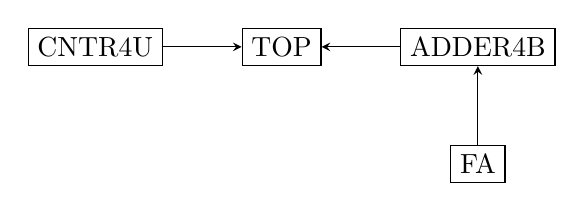
\begin{tikzpicture}[>=stealth]
        \node[draw] (cntr4u) {CNTR4U};
        \node[draw, right=of cntr4u] (top) {TOP};
        \draw[->] (cntr4u) -- (top);
        \node[draw, right=of top] (adder4b) {ADDER4B};
        \draw[<-] (top) -- (adder4b);
        \node[draw, below=of adder4b] (fa) {FA};
        \draw[<-] (adder4b) -- (fa);
    \end{tikzpicture}
    \caption{4位无符号数乘法器顶层模块设计图}
\end{figure}

具体逻辑如下

\begin{lstlisting}[language=Verilog, caption={4位无符号数乘法器顶层模块}]
module mul (
    input  wire       CLK,
    input  wire       RST,
    input  wire [3:0] X,
    input  wire [3:0] Y,
    output wire [7:0] Z
);

  wire [3:0] Q;
  wire LOAD = (Q == 4'd0);
  wire STOP = (Q == 4'd5);

  CNTR4U counter (
      .clk(CLK),
      .CLR(RST),
      .LD (1'b0),
      .ENP(~STOP),
      .ENT(~STOP),
      .D  (4'b0000),
      .Q  (Q),
  );

  reg  [3:0] P;
  reg  [3:0] Y_reg;
  wire [3:0] S;
  wire       Cout;

  assign {Cout, S} = P + (Y_reg[0] ? X : 4'd0);

  always @(posedge CLK or posedge RST) begin
    if (RST) begin
      P     <= 4'b0000;
      Y_reg <= 4'b0000;
    end else if (LOAD) begin
      P     <= 4'b0000;
      Y_reg <= Y;
    end else if (!STOP) begin
      P     <= {Cout, S[3:1]};
      Y_reg <= {S[0], Y_reg[3:1]};
    end
  end

  assign Z = {P, Y_reg};

endmodule
\end{lstlisting}

\begin{table}[H]
    \centering
    \begin{tabular}{|c|c|}
        \hline
        引脚 & 功能 \\
        \hline
        CLK & 时钟信号 \\
        RST & 异步复位 \\
        X   & 4位无符号数输入 \\
        Y   & 4位无符号数输入 \\
        Z   & 8位无符号数输出 (乘积) \\
        \hline
    \end{tabular}
    \caption{4位无符号数乘法器引脚功能表}
\end{table}

\subsection{电路设计}

\begin{figure}[H]
    \centering
    \subcaptionbox{原理图}{
        \begin{circuitikz}[>=stealth]
            \node[ALU, rotate=-90, muxdemux def={NB=1}] (alu) at (0,0) {};
            \node[draw, above] at (alu.lpin 1) {X};
            \node[draw] (P) at (0,-1.5) {P};
            \node[draw] (Y) at (1.2,-1.5) {Y};
            \node[draw] (Cout) at (-1.5,-1.5) {Cout};
            \draw (alu.rpin 1) -- (P);
            \draw (alu.bpin 1) -- (Cout.north -| alu.bpin 1);
            \draw[->] (Cout) -- (P);
            \draw[->] (P) -- (Y);
            \node[draw] (cnt) at (3,-1.5) {CNTR4U};
            \draw[<-] (Y) -- (cnt);
            \draw[->] (Y) -- ++(0,-0.8) -| (cnt);
            \draw[->] (cnt) |- (alu.tpin 1);
            \draw[->] (P) |- ++(-3,-0.8) |- (alu.lpin 2);
        \end{circuitikz}
    }
    \subcaptionbox{电路图}{
\includegraphics[width=0.9\textwidth]{assets/exp3/circuit.png}}
    \caption{4位无符号数乘法器电路设计}
\end{figure}

这里与实验报告的实现有所不同。实验报告中使用了一个桶形移位器，
但由于这里只固定的需要移动一位，桶形移位器放在这里可以说是大材小用了；
并且如果使用桶形移位器，需要对其中的内部实现进行修改，
添加一个新的输入使其满足实验的需求，这样就增加了电路的复杂度，
我认为不太合适。所以这里我采用了分线器来实现移位操作，逻辑更直白。

\subsection{仿真结果}

\begin{figure}[H]
    \centering
    
\includegraphics[width=\textwidth]{assets/exp3/sim1.png}
    \caption{4位无符号数乘法器仿真结果(a)}
\end{figure}

\begin{figure}[H]
    \centering
    
\includegraphics[width=\textwidth]{assets/exp3/sim2.png}
    \caption{4位无符号数乘法器仿真结果(b)}
\end{figure}

\begin{figure}[H]
    \centering
    
\includegraphics[width=\textwidth]{assets/exp3/sim3.png}
    \caption{4位无符号数乘法器仿真结果(c)}
\end{figure}

\begin{figure}[H]
    \centering
    
\includegraphics[width=\textwidth]{assets/exp3/sim4.png}
    \caption{4位无符号数乘法器仿真结果(d)}
\end{figure}

\begin{figure}[H]
    \centering
    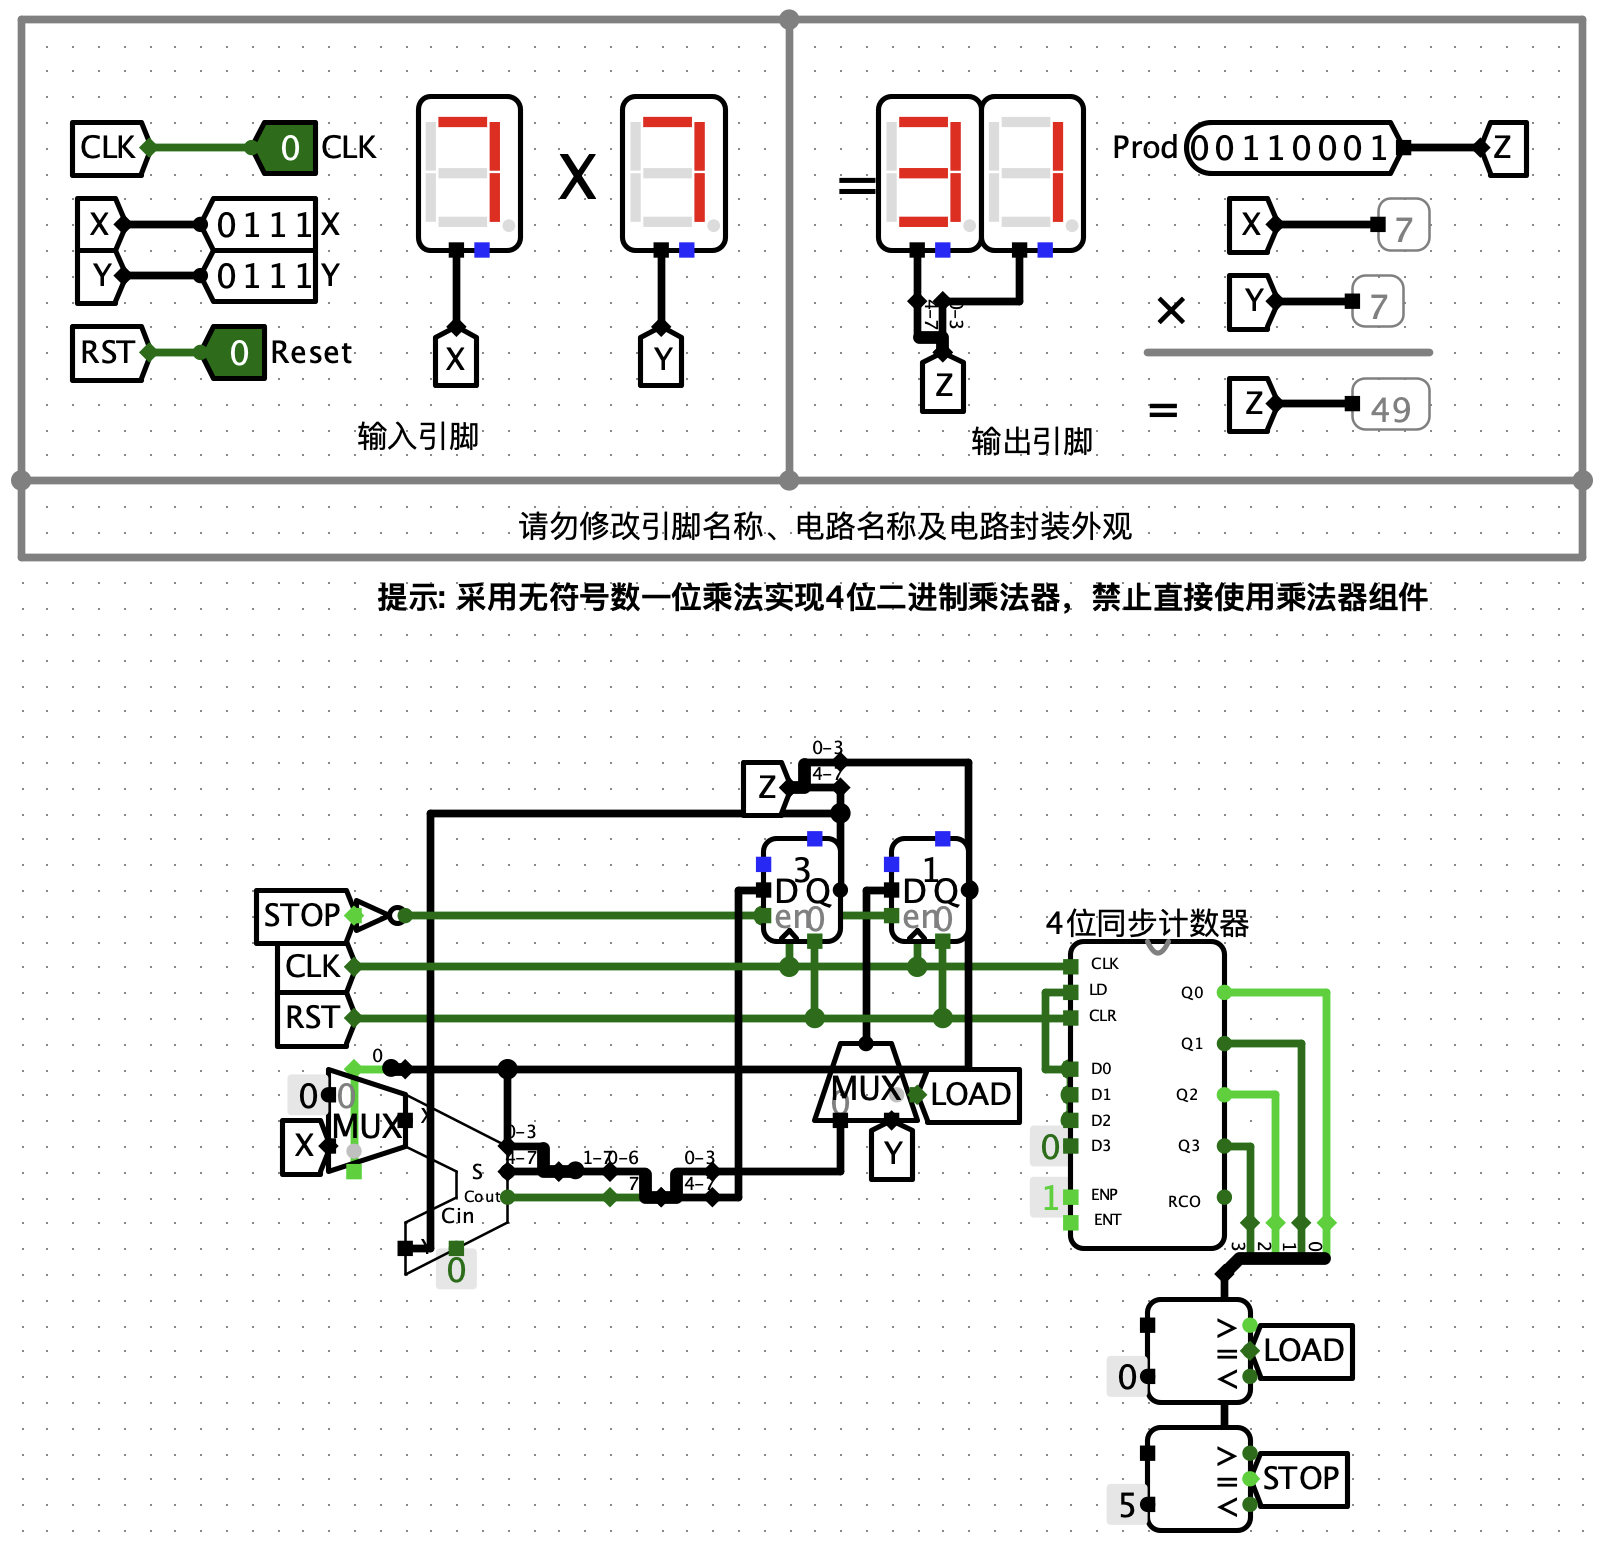
\includegraphics[width=0.9\textwidth]{assets/exp3/sim5.png}
    \caption{4位无符号数乘法器仿真结果(e)}
\end{figure}

由于真值表过于复杂，这里只取部分数据展示。

\begin{table}[H]
    \centering
    \begin{tabular}{|ccccc|ccccc|}
        \hline
        Cnt & Reset & X & Y & Z & Cnt & Reset & X & Y & Z \\
        \hline
        0 & 1 & 7 & 7 & 00 & 0 & 1 & f & f & 00 \\
        1 & 0 & 7 & 7 & 00 & 1 & 0 & f & f & 00 \\
        2 & 0 & 7 & 7 & 07 & 2 & 0 & f & f & 0f \\
        3 & 0 & 7 & 7 & 3b & 3 & 0 & f & f & 7f \\
        4 & 0 & 7 & 7 & 55 & 4 & 0 & f & f & b7 \\
        5 & 0 & 7 & 7 & 62 & 5 & 0 & f & f & d3 \\
        6 & 0 & 7 & 7 & 31 & 6 & 0 & f & f & e1 \\
        7 & 0 & 7 & 7 & 31 & 7 & 0 & f & f & e1 \\
        \hline
    \end{tabular}
    \caption{4位无符号数乘法器真值表}
\end{table}

\subsection{错误现象及分析}

我在最开始做实验的时候没有读实验手册，直接按照在线评测平台的说明写的，
便没有注意到这里的桶形移位器需要经过修改，所以无法处理加法器有溢出的情况。
我在群里提出问题后才意识到自己的错误，才按照实验手册的要求修改了电路，才得以完成实验。

后来我也意识到，虽然按照实验手册的要求修改了电路，但实验手册的设计并不合理，
修改并不是一个好的解决方案，反而增加了电路的复杂度。于是我又按照自己的想法重新设计了电路，
使用了分线器来实现移位操作，逻辑更直白，电路结构更清晰。

\begin{table}[H]
    \centering
    \begin{tabular}{|ccccc|ccccc|}
        \hline
        \multicolumn{5}{|c|}{预期输出} & \multicolumn{5}{c|}{实际输出} \\
        \hline
        Cnt & Reset & X & Y & Z & Cnt & Reset & X & Y & Z \\
        \hline
        0 & 1 & f & f & 00 & 0 & 1 & f & f & 00 \\
        1 & 0 & f & f & 00 & 1 & 0 & f & f & 00 \\
        2 & 0 & f & f & 0f & 2 & 0 & f & f & 0f \\
        3 & 0 & f & f & 7f & 3 & 0 & f & f & 7f \\
        4 & 0 & f & f & \textbf{b7} & 4 & 0 & f & f & \textbf{37} \\
        5 & 0 & f & f & \textbf{d3} & 5 & 0 & f & f & \textbf{13} \\
        6 & 0 & f & f & \textbf{e1} & 6 & 0 & f & f & \textbf{01} \\
        6 & 0 & f & f & \textbf{e1} & 6 & 0 & f & f & \textbf{01} \\
        \hline
    \end{tabular}
    \caption{4位无符号数乘法器错误现象分析表}
\end{table}

\section{实验四：寄存器堆实验}

\subsection{整体方案设计}

本实验为单模块，逻辑如下

\begin{lstlisting}[language=Verilog, caption={寄存器堆模块}]
module regfile (
    input  wire        clk,
    input  wire        WE,
    input  wire [ 4:0] RW,
    input  wire [ 4:0] RA,
    input  wire [ 4:0] RB,
    input  wire [31:0] Din,
    output wire [31:0] RDA,
    output wire [31:0] RDB
);

  reg [31:0] registers[31:0];

  assign RDA = registers[RA];
  assign RDB = registers[RB];

  always @(posedge clk) begin
    if (WE) registers[RW] <= Din;
  end

endmodule
\end{lstlisting}

在 Logisim 中，需要使用解码器来实现寄存器选择的功能，使用多路选择器来实现寄存器输出的功能。

\begin{table}[H]
    \centering
    \begin{tabular}{|c|c|}
        \hline
        引脚 & 功能 \\
        \hline
        clk & 时钟信号 \\
        WE  & 写使能 (高电平有效) \\
        RW  & 寄存器写地址 (5位) \\
        RA  & 寄存器读地址 A (5位) \\
        RB  & 寄存器读地址 B (5位) \\
        Din & 数据输入 (32位) \\
        RDA & 数据输出 A (32位) \\
        RDB & 数据输出 B (32位) \\
        \hline
    \end{tabular}
    \caption{寄存器堆引脚功能表}
\end{table}

\subsection{电路设计}

由于电路图高度超限，这里只截取部分电路。

同样，中间的寄存器只取了 $Reg_k(0\le k\le 31)$ 来表示。

\begin{figure}[H]
    \centering
    \subcaptionbox{原理图}{
        \begin{circuitikz}
            \node[
                muxdemux,
                muxdemux def={Lh=1, Rh=3, NL=1, NB=1, NR=3},
                muxdemux label={R1=0, R2=k, R3=31, B1=En},
                draw only right pins={2}
            ] (decoder) at (0,0) {};
            \node[left] at (decoder.lpin 1) {RW};
            \node[below] at (decoder.bpin 1) {WE};
            \node[
                flipflop JK,
                flipflop def={t1=EN, t3=D, t4=},
                anchor=pin 1
            ] (reg) at (2,0) {$Reg_k$};
            \node[left] at (reg.pin 2) {Clk};
            \node[left] at (reg.pin 3) {$Din_k$};
            \draw (decoder.rpin 2) -- (reg.pin 1);
            \node[
                muxdemux,
                muxdemux def={Lh=3, Rh=1, NL=3, NB=1, NR=1},
                muxdemux label={L1=0, L2=k, L3=31},
                draw only left pins={2}
            ] (mux1) at (6,0) {};
            \node[right] at (mux1.rpin 1) {RDA};
            \node[below] at (mux1.bpin 1) {RA};
            \draw (reg.pin 6) -- (mux1.lpin 2);
            \node[
                muxdemux,
                muxdemux def={Lh=3, Rh=1, NL=3, NB=1, NR=1},
                muxdemux label={L1=0, L2=k, L3=31},
                draw only left pins={2}
            ] (mux2) at (6,-2.5) {};
            \node[right] at (mux2.rpin 1) {RDB};
            \node[below] at (mux2.bpin 1) {RB};
            \draw (reg.pin 6) node[circ]{} |- (mux2.lpin 2);
        \end{circuitikz}
    }
    \subcaptionbox{电路图}{
\includegraphics[width=\textwidth]{assets/exp4/circuit.png}}
    \caption{寄存器堆电路设计}
\end{figure}

这里我的实现与实验手册有些许不同。由于 Logisim 支持解码器的使能端，
并设置未激活时输出零，所以可以直接用这个使能端来替代手册中 32 个与门的作用。

\subsection{仿真结果}

由于电路图高度超限，这里仿真截图只截取输入输出部分。

\begin{figure}[H]
    \centering
    
\includegraphics[width=\textwidth]{assets/exp4/sim1.png}
    \caption{寄存器堆仿真结果(a)}
\end{figure}

\begin{figure}[H]
    \centering
    
\includegraphics[width=\textwidth]{assets/exp4/sim2.png}
    \caption{寄存器堆仿真结果(b)}
\end{figure}

\begin{figure}[H]
    \centering
    
\includegraphics[width=\textwidth]{assets/exp4/sim3.png}
    \caption{寄存器堆仿真结果(c)}
\end{figure}

\begin{figure}[H]
    \centering
    
\includegraphics[width=\textwidth]{assets/exp4/sim4.png}
    \caption{寄存器堆仿真结果(d)}
\end{figure}

由于真值表过于复杂，这里只取部分数据展示。

\begin{table}[H]
    \centering
    \begin{tabular}{|c|c|c|c|c|c|c|c|c|}
        \hline
        Cnt & WE & RW & RA & RB & Din & RDA & RDB \\
        \hline
        00 & 1 & 00 & 00 & 00 & 00000001 & 00000000 & 00000000 \\
        01 & 1 & 01 & 00 & 00 & 005deece & 00000001 & 00000001 \\
        02 & 1 & 02 & 00 & 01 & b61488df & 00000001 & 005deece \\
        03 & 1 & 03 & 01 & 02 & f4111591 & 005deece & b61488df \\
        04 & 1 & 04 & 02 & 03 & 023eaf12 & b61488df & f4111591 \\
        05 & 1 & 05 & 03 & 04 & b578fa6a & f4111591 & 023eaf12 \\
        06 & 1 & 06 & 04 & 05 & d38a8b1c & 023eaf12 & b578fa6a \\
        07 & 1 & 07 & 05 & 06 & f5d50649 & b578fa6a & d38a8b1c \\
        08 & 1 & 08 & 06 & 07 & 202e3c08 & d38a8b1c & f5d50649 \\
        09 & 1 & 09 & 07 & 08 & 812fba12 & f5d50649 & 202e3c08 \\
        \hline
    \end{tabular}
    \caption{寄存器堆真值表}
\end{table}

\subsection{错误现象及分析}

在完成实验的过程中，没有遇到任何错误。

\newpage

\section{实验五：数字时钟实验}

\subsection{整体方案设计}

本实验的代码实验为单模块，逻辑如下

\begin{lstlisting}[language=Verilog, caption={数字时钟模块}]
module clock (
    input wire CLK,
    input wire LD,

    input wire [3:0] HH1,
    input wire [3:0] HH0,
    input wire [3:0] MM1,
    input wire [3:0] MM0,
    input wire [3:0] SS1,
    input wire [3:0] SS0,

    output reg [3:0] H1,
    output reg [3:0] H0,
    output reg [3:0] M1,
    output reg [3:0] M0,
    output reg [3:0] S1,
    output reg [3:0] S0,

    output wire LED_R,
    output wire LED_G,
    output wire LED_B,

    output wire INErr
);

  wire valid_HH = (HH1 < 2 && HH0 <= 9) || (HH1 == 2 && HH0 <= 3);
  wire valid_MM = (MM1 <= 5 && MM0 <= 9);
  wire valid_SS = (SS1 <= 5 && SS0 <= 9);
  wire time_valid = valid_HH && valid_MM && valid_SS;

  wire LD_EN = LD && time_valid;
  assign INErr = LD && !time_valid;

  wire C_S0 = (S0 == 9);
  wire C_S1 = (S1 == 5 && C_S0);
  wire C_M0 = (M0 == 9 && C_S1);

  wire LED_EN = (M1 == 5 && C_M0);
  wire C_H0 = (H0 == 9 && LED_EN);
  wire C_24H = (H1 == 2 && H0 == 3 && LED_EN);

  reg [3:0] cnt;
  wire START = (cnt != 0);

  always @(posedge CLK) begin
    if (LD_EN) begin
      S0  <= SS0;
      S1  <= SS1;
      M0  <= MM0;
      M1  <= MM1;
      H0  <= HH0;
      H1  <= HH1;
      cnt <= 0;
    end else begin
      if (C_S0) S0 <= 0;
      else S0 <= S0 + 1;

      if (C_S1) S1 <= 0;
      else if (C_S0) S1 <= S1 + 1;

      if (C_M0) M0 <= 0;
      else if (C_S1) M0 <= M0 + 1;

      if (LED_EN) M1 <= 0;
      else if (C_M0) M1 <= M1 + 1;

      if (C_24H) H0 <= 0;
      else if (C_H0) H0 <= 0;
      else if (LED_EN) H0 <= H0 + 1;

      if (C_24H) H1 <= 0;
      else if (C_H0) H1 <= H1 + 1;

      if (LED_EN) begin
        cnt <= 1;
      end else if (START) begin
        if (cnt == 10) cnt <= 0;
        else cnt <= cnt + 1;
      end
    end
  end

  assign LED_R = START ? (cnt[0] ^ cnt[1]) : 0;
  assign LED_G = START ? (cnt[1] ^ cnt[2]) : 0;
  assign LED_B = START ? cnt[2] : 0;

endmodule
\end{lstlisting}

\begin{table}[H]
    \centering
    \begin{tabular}{|c|c|c|c|}
        \hline
        引脚 & 功能 & 引脚 & 功能 \\
        \hline
        CLK & 时钟信号               & LED\_R & 红色LED输出 (高电平有效) \\
        LD  & 载入时间信号 (高电平有效) & LED\_G & 绿色LED输出 (高电平有效) \\
        INErr & 输入错误指示          & LED\_B & 蓝色LED输出 (高电平有效) \\
        \hline
        HH1 & 小时十位输入 (4位二进制) & H1  & 小时十位输出 (4位二进制) \\
        HH0 & 小时个位输入 (4位二进制) & H0  & 小时个位输出 (4位二进制) \\
        MM1 & 分钟十位输入 (4位二进制) & M1  & 分钟十位输出 (4位二进制) \\
        MM0 & 分钟个位输入 (4位二进制) & M0  & 分钟个位输出 (4位二进制) \\
        SS1 & 秒钟十位输入 (4位二进制) & S1  & 秒钟十位输出 (4位二进制) \\
        SS0 & 秒钟个位输入 (4位二进制) & S0  & 秒钟个位输出 (4位二进制) \\
        \hline
    \end{tabular}
\end{table}

\subsection{电路设计}

以下为主要部分的原理图

\begin{figure}[H]
    \centering
    \begin{circuitikz}
        \node[
            flipflop JK,
            flipflop def={t1=D, t3=En, t4=, tu=LD, td=0}
        ] (h0) at (0,0) {};
        \node[
            flipflop JK,
            flipflop def={t1=D, t3=En, t4=, tu=LD, td=0}
        ] (m0) at (4.5,0) {};
        \node[
            flipflop JK,
            flipflop def={t1=D, t3=En, t4=, tu=LD, td=0}
        ] (s0) at (9,0) {};
        \node[
            flipflop JK,
            flipflop def={t1=D, t3=En, t4=, tu=LD, td=0}
        ] (h1) at (0,-4) {};
        \node[
            flipflop JK,
            flipflop def={t1=D, t3=En, t4=, tu=LD, td=0}
        ] (m1) at (4.5,-4) {};
        \node[
            flipflop JK,
            flipflop def={t1=D, t3=En, t4=, tu=LD, td=0}
        ] (s1) at (9,-4) {};
        \node[left] at (h0.pin 1) {HH0};
        \node[left] at (h1.pin 1) {HH1};
        \node[left] at (m0.pin 1) {MM0};
        \node[left] at (m1.pin 1) {MM1};
        \node[left] at (s0.pin 1) {SS0};
        \node[left] at (s1.pin 1) {SS1};
        \node[left] at (h0.pin 2) {CLK};
        \node[left] at (h1.pin 2) {CLK};
        \node[left] at (m0.pin 2) {CLK};
        \node[left] at (m1.pin 2) {CLK};
        \node[left] at (s0.pin 2) {CLK};
        \node[left] at (s1.pin 2) {CLK};
        \node[left] at (h0.pin 3) {C\_M1};
        \node[left] at (h1.pin 3) {C\_H0};
        \node[left] at (m0.pin 3) {C\_S1};
        \node[left] at (m1.pin 3) {C\_M0};
        \node[left] at (s0.pin 3) {1};
        \node[left] at (s1.pin 3) {C\_S0};
        \node[above] at (h0.up) {LD\_EN};
        \node[above] at (h1.up) {LD\_EN};
        \node[above] at (m0.up) {LD\_EN};
        \node[above] at (m1.up) {LD\_EN};
        \node[above] at (s0.up) {LD\_EN};
        \node[above] at (s1.up) {LD\_EN};
        \node[below] at (h0.down) {CLR\_H0};
        \node[below] at (h1.down) {CLR\_H1};
        \node[below] at (m0.down) {C\_M0};
        \node[below] at (m1.down) {C\_M1};
        \node[below] at (s0.down) {C\_S0};
        \node[below] at (s1.down) {C\_S1};
        \node[right] at (h0.pin 6) {H0};
        \node[right] at (h1.pin 6) {H1};
        \node[right] at (m0.pin 6) {M0};
        \node[right] at (m1.pin 6) {M1};
        \node[right] at (s0.pin 6) {S0};
        \node[right] at (s1.pin 6) {S1};
    \end{circuitikz}
    \caption{数字时钟原理图(a)}
\end{figure}

其中，需要用比较器或者组合逻辑来实现

\begin{itemize}
    \item $C_{S0} = (S0 == 9)$
    \item $C_{S1} = (S1 == 5) \land C_{S0}$
    \item $C_{M0} = (M0 == 9) \land C_{S1}$
    \item $C_{M1} = (M1 == 5) \land C_{M0}$
    \item $C_{H0} = (H0 == 9) \land C_{M1}$
    \item $CLR_{H1} = (H1 == 2) \land (H0 == 3) \land C_{M1}$
    \item $CLR_{H0} = C_{H0} \lor CLR_{H1}$
    \item $LED_{EN} = C_{M0} \land C_{M1} \land C_{S0} \land C_{S1}$
    \item $LD_{EN} = LD \land (\lnot INErr)$
    \item $INErr = LD \land (
        ((HH_1 < 2 \land HH_0 < 10) \lor (HH_1 == 2 \land HH_0 < 4))
        \newline \land (MM_1 < 6 \land MM_0 < 10)
        \land (SS_1 < 6 \land SS_0 < 10))$
\end{itemize}

\newpage

以下为 LED 部分的原理图

\begin{figure}[H]
    \centering
    \begin{circuitikz}
        \node[
            flipflop JK,
            flipflop def={t1=D, t3=En, t4=, tu=LD, td=0}
        ] (cnt) at (0,0) {};
        \node[left] at (cnt.pin 1) {1};
        \node[left] at (cnt.pin 2) {CLK};
        \node[left] at (cnt.pin 3) {START};
        \node[above] at (cnt.up) {LED\_EN};
        \node[below] at (cnt.down) {STOP};
        \node[right] at (cnt.pin 6) {Cnt};
    \end{circuitikz}
    \caption{数字时钟原理图(b)}
\end{figure}

其中，需要用比较器或者组合逻辑来实现

\begin{itemize}
    \item $START = (Cnt \ne 0)$
    \item $STOP = (Cnt \le 10)$
    \item $LED_R = START \land (Cnt[0] \oplus Cnt[1])$
    \item $LED_G = START \land (Cnt[1] \oplus Cnt[2])$
    \item $LED_B = START \land Cnt[2]$
\end{itemize}

\begin{figure}[H]
    \centering
    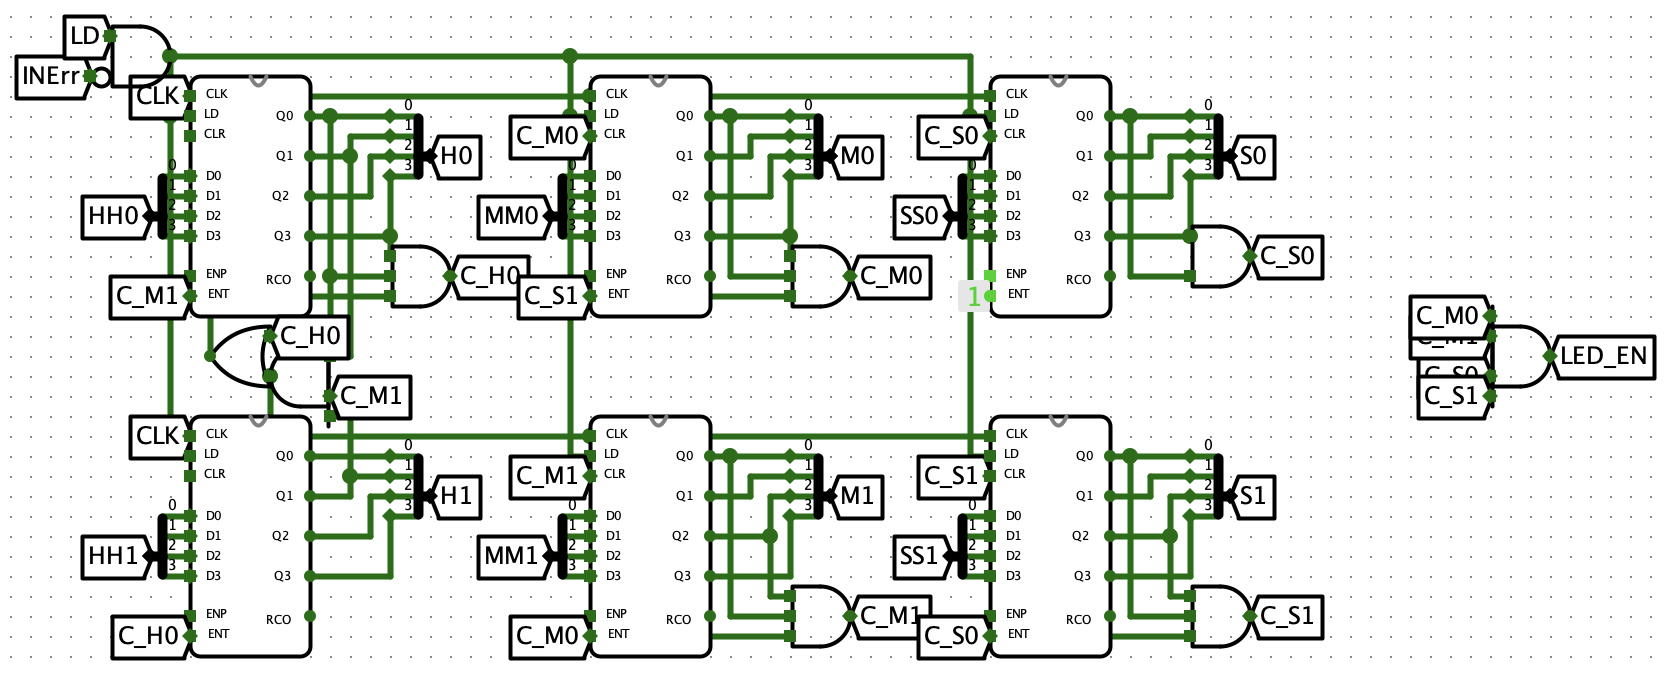
\includegraphics[width=\textwidth]{assets/exp5/circuit1.png}
    \caption{数字时钟电路图(a)}
\end{figure}

\begin{figure}[H]
    \centering
    \subcaptionbox*{(b)}{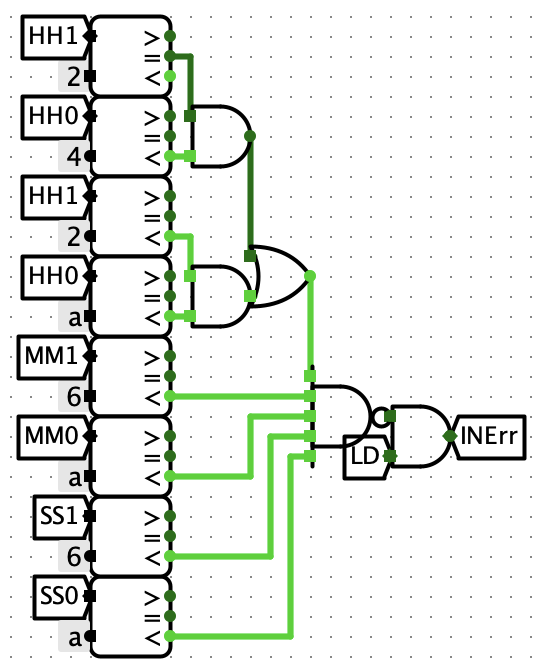
\includegraphics[width=0.3\textwidth]{assets/exp5/circuit2.png}}
    \subcaptionbox*{(c)}{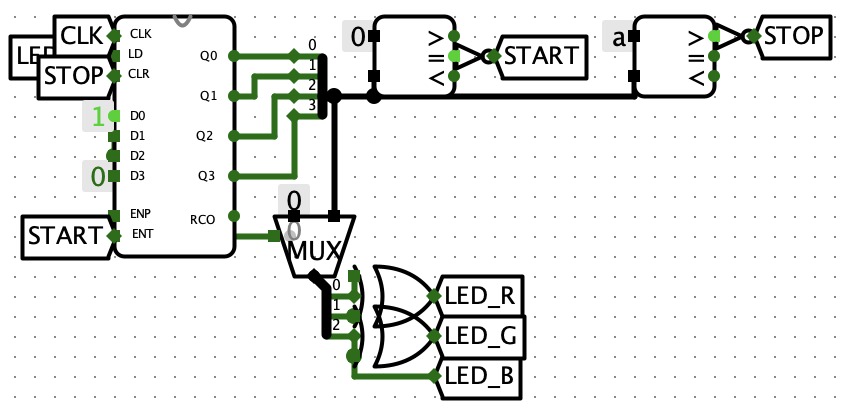
\includegraphics[width=0.65\textwidth]{assets/exp5/circuit3.png}}
    \caption{数字时钟电路图}
\end{figure}

\subsection{仿真结果}

\begin{figure}[H]
    \centering
    
\includegraphics[width=\textwidth]{assets/exp5/sim1.png}
    \caption{数字时钟仿真结果(a)}
\end{figure}

\begin{figure}[H]
    \centering
    
\includegraphics[width=\textwidth]{assets/exp5/sim2.png}
    \caption{数字时钟仿真结果(b)}
\end{figure}

\begin{figure}[H]
    \centering
    
\includegraphics[width=\textwidth]{assets/exp5/sim3.png}
    \caption{数字时钟仿真结果(c)}
\end{figure}

其中，LED 输出的真值表为

\begin{table}[H]
    \centering
    \begin{tabular}{|c|c|c|c|}
        \hline
        Cnt & LED\_R & LED\_G & LED\_B \\
        \hline
        0 & 0 & 0 & 0 \\
        1 & 1 & 0 & 0 \\
        2 & 1 & 1 & 0 \\
        3 & 0 & 1 & 0 \\
        4 & 0 & 1 & 1 \\
        5 & 1 & 1 & 1 \\
        6 & 1 & 0 & 1 \\
        7 & 0 & 0 & 1 \\
        8 & 0 & 0 & 0 \\
        \hline
    \end{tabular}
    \caption{数字时钟LED输出真值表}
\end{table}

\subsection{错误现象及分析}

最开始我化简 INErr 的表达式有误，虽然通过了在线平台的测试，但我在检查时发现了异常。

\begin{figure}[H]
    \centering
    \subcaptionbox{错误的电路图}{
\includegraphics[width=0.4\textwidth]{assets/exp5/error.png}}
    \subcaptionbox{正确的电路图}{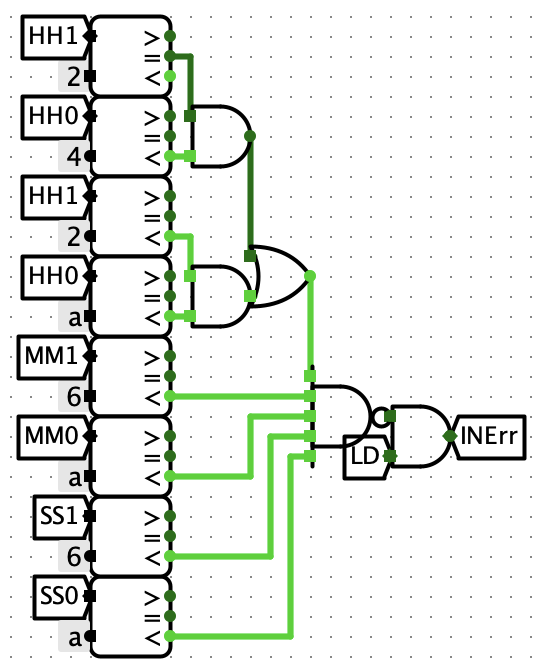
\includegraphics[width=0.4\textwidth]{assets/exp5/circuit2.png}}
    \caption{数字时钟实验中出现的错误}
\end{figure}

\end{document}
